\documentclass{article}

%packages

\usepackage[utf8]{inputenc}
\usepackage[french]{babel}
\usepackage{graphicx}
\usepackage{hyperref}
\RequirePackage{fix-cm}
\usepackage{mwe}
\usepackage[margin=2cm]{geometry}
\usepackage[linesnumbered,ruled]{algorithm2e}
\usepackage{float}
\usepackage{caption}
\usepackage{tikz}
\usepackage{xcolor}
\usepackage{listings}
\lstset{basicstyle=\ttfamily,
  showstringspaces=false,
  commentstyle=\color{red},
  keywordstyle=\color{blue}
}


%commandes
\newcommand{\size}[2]{{\fontsize{#1}{0}\selectfont#2}}
\newenvironment{sizepar}[2]
 {\par\fontsize{#1}{#2}\selectfont}
 {\par}

\begin{document}
\begin{titlepage}
	\parindent0pt
	\hskip.25cm \vrule width.8pt \hskip.25cm
	\vskip0pt plus 1fil
	\fbox{%
		\begin{minipage}{\dimexpr\linewidth-2\fboxsep-2\fboxrule}
			\centering\Large\bfseries
			\vskip1cm
			Corpus
			\vskip1cm \kern0pt
		\end{minipage}%
	}%
	\vskip0.5cm
	\centerline{\textbf{Données Web}}
	\vskip0pt plus 1fil
	\vskip0.25cm
	\centerline{HUET Bryan, SAHIN Tolga}
	\leavevmode
	\vskip0pt plus 2fil
	\hfill\bfseries{Année universitaire 2020}\hfill\null
\end{titlepage}

\tableofcontents
\newpage

\section{Introduction}

Le projet de notre corpus est de réaliser un moteur de recherche via des indexage et à l'aide la méthode de pondération TF-IDF.



\subsection{Le TF-IDF}

Le tf-idf est le poids d'un mot dans un ensemble de documents. Ce poids augmentera en fonction de la fréquence brute des mots (TF) et de la fréquence des mots dans tous les documents. (DF)
Si le tf-idf est grand alors plus le mot est fréquent. Tandis que, moins il l'est le mot est peu fréquent.

\subsection{Indexage}

Le second objectif ce ce projet est de rechercher la fréquence (TF-IDF) de différents mots dans un paquet de documents. De ce fait-là, nous procéderons à un indexage à l'aide de différentes requêtes. Puis, nous calculerons le TF-IDF des mots.

\section{Calcul du TF}

\subsection{Le TF}

Le TF est la fréquence des mots dans un document. (Term Frequency)

\subsection{Calcul du TF}

On commence par récupérer l'ensemble de nos documents (3655 dans notre cas).

\begin{lstlisting}[language=bash,caption={Bouclage}]
for i in $(seq 3655) ; do cat $i | ...
\end{lstlisting}

On convertit tous nos String majuscule en miniscule.

\begin{lstlisting}[language=bash,caption={Miniscule}]
tr [:upper:] [:lower:] | ...
\end{lstlisting}

On transforme tous les mots qui utilise des caractères spéciaux, des espaces et des sauts de ligne.

\begin{lstlisting}[language=bash,caption={Caractères spéciaux}]
sed 's/[^a-z]/ /g' | sed 's/ /\n/g' | ...
\end{lstlisting}


Si le nombre de fields est différent de 0 alors on print les champs de texte. Puis, on pipe l'output avec la requête sort qui permet de trier. Donc, on obtient une liste de mot ordonnée.

\begin{lstlisting}[language=bash,caption={Liste de mots triés}]
awk 'NF != 0 {print}'| sort | ...
\end{lstlisting}

La requête awk permet de calculer le TF. On calcule depuis notre liste de mots. Le nombre d'occurrences de chacun de ces mots. On retourne le mot et son TF.
La requête sed permet de supprimer la première ligne avec le paramètre '1d'. Puis, de stocker les résultats du script (les TF des mots) dans des fichiers .tf jusqu'à la fin de notre boucle.

\begin{lstlisting}[language=bash,caption={Calcul du TF}]
awk '{if (mot == $1) tf ++; 
else {print mot, tf; mot = $1; tf = 1}} END {print mot, tf}' 
| sed 1d >$i.tf;done
\end{lstlisting}

\subsection{Temps d'exécution avec time}

Le script TF prend en moyenne à l'aide la requête time ce délai :

\begin{lstlisting}[language=bash,caption={Suppression}]
time bash df.sh

real 1m18,654s
user 1m0,027s
sys 0m28,940s
\end{lstlisting}

\subsection{Temps d'exécution avec usr/bin/time}
\label{labeltime}

Temps d'exécution cette fois-ci calculer avec usr/bin/time.

Pour que cela marche, on passe sur nos script sur un bouclage variable :
\begin{lstlisting}[language=bash,caption={Bouclage variable}]

j=$1
for i in ($(seq $((j * 500))); do ...

\end{lstlisting}

En terminal nous lancerons de cette manière notre script.
Les temps d'exécutions vont être écrites sur un fichier "resultat.txt". Ainsi, on pourra utiliser gnuplot pour observer ceci depuis un graphe.

\begin{lstlisting}[language=bash,caption={Requête d'exécution}]

for j in $(seq 7); do usr/bin/time -p -o ../resultat.txt -a bash tf.sh $j; done

\end{lstlisting}

\subsection{Graphique avec gnuplot}

On récupère uniquement les valeurs de real avec la requête awk suivante.
 
\begin{lstlisting}[language=bash,caption={Fichier à plot}]
awk '/real/{print $2}' resultat.txt > tf.txt
\end{lstlisting}


\begin{figure}[H]
\centering
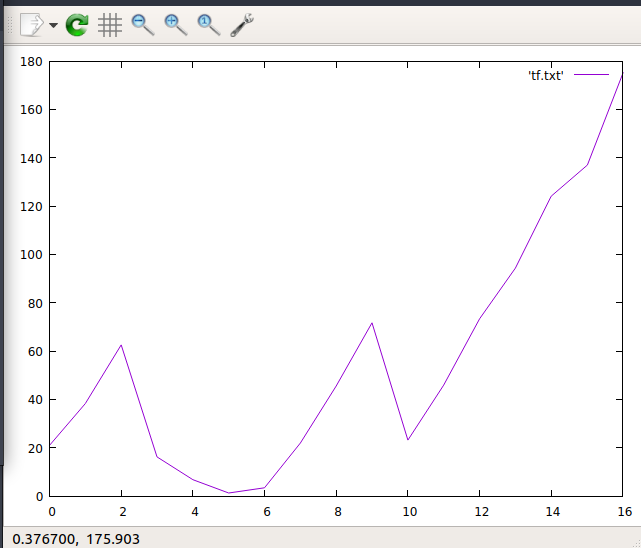
\includegraphics[scale = 0.5]{"img/tf.png"}
\caption{Graphique du temps d'exécution du script tf.sh}
\end{figure}

Au début, mon temps d'exécution est variable mais sur la fin de la boucle il est presque linéaire.

\section{Le DF}

\subsection{Définition}

Le DF (Document Frequency) est le nombre d'occurence de tous les mots dans un ensemble de documents.

\subsection{Calcul du DF}

Le début du script suit exactement le même principe que pour le TF.

\begin{lstlisting}[language=bash,caption={Bouclage}]
for i in $(seq 3655); do cat $i 
| tr [:upper:] [:lower:]
| sed 's/[^a-z]/ /g' 
| sed 's/ /\n/g' | ...
\end{lstlisting}

sort -u est aussi équivalent à sort | uniq.
Ce paramètre permet de trier plus efficacement notre ensemble de documents. Les mots dupliqués sont éliminés. Donc, notre output devient la liste de mot de l'ensemble des documents. De plus, "done;" est important car il ferme notre boucle pour ne garder en sortie que cette liste de mot.
On trie cette liste de mot cette fois-ci via la requête sort. On obtient une liste de mots par ordre alphabétique.

\begin{lstlisting}[language=bash,caption={Tris}]
awk 'NF != 0 {print}'| sort -u; done | sort | ...
\end{lstlisting}

Enfin, on termine le script de la même manière que pour le TF. On compte le nombre d'occurrence de notre liste de mot. Sauf que cette fois-ci notre output est stocké dans un seul fichier texte "df.txt" car on ne boucle plus. Cette output contient le mot et la fréquence de mot par ligne. Donc, l'output est le DF des mots dans nos documents.

\begin{lstlisting}[language=bash,caption={Occurences}]
awk '{if (mot == $1) tf ++; 
else {print mot, tf; mot = $1; tf = 1}} END {print mot, tf}' 
| sed 1d > ../df.txt
\end{lstlisting}

\subsection{Temps d'exécution}

\begin{lstlisting}[language=bash,caption={Temps d'exécution du script df.sh}]
time bash df.sh

real 1m1.042s
user 0m51,006s
sys 0m28,940s

\end{lstlisting}

\subsection{Temps d'exécution avec usr/bin/time}

On fait la même chose que dans la partie \ref{labeltime} pour le TF.

\subsection{Graphe avec gnuplot}

\begin{figure}[H]
\centering
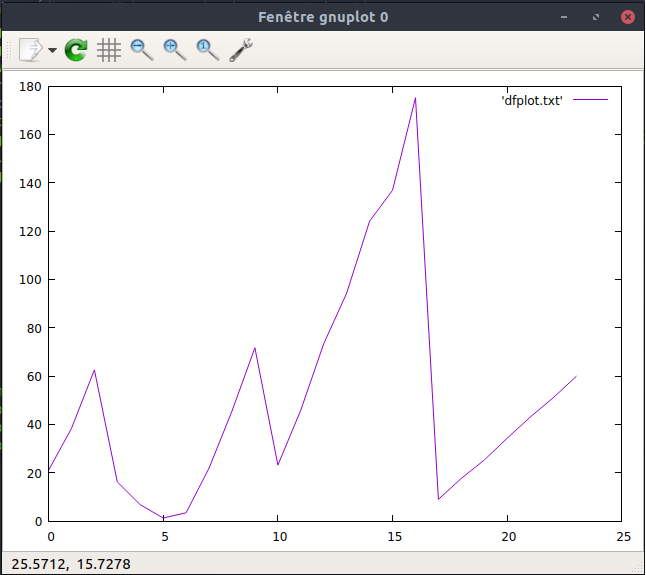
\includegraphics[scale = 0.5]{"img/df.png"}
\caption{Graphique du temps d'exécution du script df.sh}
\end{figure}

Les temps d'exécutions sont variables sur certains instants. Mais, il y'a de la linéarité
comme pour le tf.

\section{Indexage et calcul du TF-IDF}

L'indexage et le calcul du TF-IDF va s'effectuer en quatre script. 

\subsection{Premier script}

On récupère le contenu des fichiers .tf (liste de mots avec le TF). On lie chaque mots à une valeur qui correspond au numéro(s) de document(s) dans lequel il s'y présente.

\begin{lstlisting}[language=bash,caption={Requête 1}]
#!/bin/bash
for i in $(seq 3655); do cat "content/"$i.tf 
| sed "s/ .*/ $i/"; done | ...
\end{lstlisting}

Tri les mots par ordre alphabétique et croissant de documents.

\begin{lstlisting}[language=bash,caption={Requête 2}]
sort -k1,1 -k2,2n | ...
\end{lstlisting}

On supprime les duplications de mots. Puis, on regroupe en une ligne tous les numéros de documents dans lequel se présente le mot.
La liste de mots et de numéros est stocké dans le fichier index.

\begin{lstlisting}[language=bash,caption={Requête 3}]
awk '{if ($1 != last){if (last!="")print last, tab[last]; last = $1; tab[last] = $2} 
else tab[last] = tab[last] " " $2}END{print last, tab[last]}' > index
\end{lstlisting}


\subsection{Second script}

On récupère les mots et les numéros de documents depuis le fichier index de nos mots dans query.
\begin{lstlisting}[language=bash,caption={Requete 1}]
for i in $(cat query.txt); do grep "^$i " index | ...
\end{lstlisting}

Recupère les numéros de documents.

\begin{lstlisting}[language=bash,caption={Requête 2}]
sed 's/[^ ]* //; s/ /\n/g' | ...
\end{lstlisting}

Tri des numéros et stockage dans des fichiers mot.index
\begin{lstlisting}[language=bash,caption={Requête 3}]
sort > $i.index; done;
\end{lstlisting}

On copie les valeurs de chaque fichier index et le stockons dans answer.

\begin{lstlisting}[language=bash,caption={Requête 4}]
cp $(head -1 query.txt).index answer;
\end{lstlisting}

On compare le fichier "answer" et les fichiers "i.index". Le paramétrage -1 supprime les lignes uniques d'answer et -2 ceux des fichiers index. Puis, stockons les lignes restantes dans tmp. On renomme tmp en answer.

\begin{lstlisting}[language=bash,caption={Requête 5}]
for i in $(sed 1d query.txt); 
do comm -1 -2 answer $i.index > tmp; mv tmp answer; done;
\end{lstlisting}

\subsection{Troisième script}

On cat query. La requête grep permet de récupérer le DF correspondant à chaque mot de query.

\begin{lstlisting}[language=bash,caption={Requête 1}]
for i in $(cat query.txt); do grep "^$i " df.txt; done | ...
\end{lstlisting}


On effectue le calcul de TF-IDF avec log(nombres de fichiers / valeurs de df). On stocke les tf-idf dans query.tfidf.

\begin{lstlisting}[language=bash,caption={Requête 2}]
awk '{print $1, log(3655/$2)}' | awk '{print $2}' > query.tfidf
\end{lstlisting}

\subsection{Quatrième script}

La première boucle récupère les numéros de documents sans duplication depuis answer.
La seconde boucle, à l'aide de la requête grep permet de relier les numéros de documents leur mot et leur tf-idf en une ligne.

\begin{lstlisting}[language=bash,caption={Requête 1}]
for i in $(sort answer); do echo -n "$i ";
for j in $(cat query); do grep "^$j " $i.tfidf | ...
\end{lstlisting}

On récupère la pertinence des mots de chaque mots dans les précédents numéros de documents (i). Puis, on stocke ce résultat dans des fichiers "i.pert".
Paste permet d'écrire les lignes tabulairement (-d) de query.tfidf et des fichiers i.pert correspondant.

\begin{lstlisting}[language=bash,caption={Requête 2}]
awk '{print $2}'; done > $i.pert; paste -d" " query.tfidf $i.pert | ...
\end{lstlisting}

On effectue le calcul sur nos valeurs comme sur la formule du TF-IDF.
Puis on supprime tous les fichiers i.pert pour de la lisibilité.

\begin{lstlisting}[language=bash,caption={Requête 3}]
awk '{sum+=$1*$2;norm1+=$1*$1;norm2+=$2*$2}END{print sum/sqrt(norm1)/sqrt(norm2)}';
rm -f $i.pert; done
\end{lstlisting}

L'output sera vu sous terminal, on observe ainsi chaque numéro de documents (où nos query apparaissent) et sa valeur de pertinence sur chaque ligne.

\subsection{Temps d'exécution avec time}

Script 1 :

\begin{lstlisting}[language=bash,caption={Temps d'exécution du script 1}]
time bash step1.sh

real 0m4,744s
user 0m6,020s
sys  0m1,207s

\end{lstlisting}

Script 2 :

\begin{lstlisting}[language=bash,caption={Temps d'exécution du script 2}]
time bash step2.sh

real 0m0,265s
user 0m0,039s
sys  0m0,008s

\end{lstlisting}

Script 3 :

\begin{lstlisting}[language=bash,caption={Temps d'exécution du script 3}]
time bash step3.sh

real 0m0,013s
user 0m0,007s
sys  0m0,012s
\end{lstlisting}

Script 4 :

\begin{lstlisting}[language=bash,caption={Temps d'exécution du script 4}]
time bash step4.sh

real 0m0,197s
user 0m0,231s
sys  0m0,071s

\end{lstlisting}

Total :

\begin{lstlisting}[language=bash,caption={Temps d'exécution en tout}]
time bash tfidf.sh

real 0m5,219s
user 0m6,297s
sys  0m1,298s

\end{lstlisting}

\section{Conclusion}

Notre moteur de recherche permet bien de récupérer depuis des mots les TF, DF, TF-IDF. Les temps d'exécutions eux varient considérablement en fonction des requêtes que l'on utilise. Notre temps d'exécution moyen nous semble correct

\end{document}